%% GENERATED by tools/from_docs.py from stepss-docs. Do not edit by hand:
%% edit the page named below in stepss-docs and regenerate.
%% source: stepss-docs/src/content/docs/models/ieee-governors.mdx

\chapter{IEEE turbine-governor models}\label{doc:model-tor-ieee}

This page documents the IEEE-standard turbine-governor models available in RAMSES, all using the \texttt{tor\_} prefix. These models implement standardised transfer-function blocks for diesel, gas-turbine, steam-turbine, hydraulic, and simplified ENTSO-E governors.

\begin{docsnote}{Usage in Dynamic Data Files}

Governor/torque models in RAMSES are defined as sub-records within a \texttt{SYNC\_MACH} block using the \texttt{TOR} keyword, followed by the model name and its parameters. They are not standalone records. The \texttt{TOR} line appears after the \texttt{EXC} (exciter) line, and the \texttt{;} at the end closes the entire \texttt{SYNC\_MACH} block.

\begin{Verbatim}
SYNC_MACH name bus FP FQ P Q SNOM Pnom H D IBRATIO
                    XT  Xl  Xd  X'd  X"d  Xq  X'q  X"q  m  n  Ra  T'do  T"do  T'qo  T"qo
              EXC model_name  param1  param2  ...
              TOR model_name  param1  param2  ... ;
\end{Verbatim}

RAMSES adds the \texttt{tor\_} prefix to the model name automatically, so both \texttt{DEGOV1} and \texttt{tor\_DEGOV1} resolve to the same model. The IEEE governor names are:

\begin{small}\begin{longtable}[]{@{}
  >{\raggedright\arraybackslash}p{(\linewidth - 8\tabcolsep) * \real{0.2299}}
  >{\raggedright\arraybackslash}p{(\linewidth - 8\tabcolsep) * \real{0.2888}}
  >{\raggedright\arraybackslash}p{(\linewidth - 8\tabcolsep) * \real{0.2785}}
  >{\raggedright\arraybackslash}p{(\linewidth - 8\tabcolsep) * \real{0.2028}}
@{}}
\toprule\noalign{}
\begin{minipage}[b]{\linewidth}\raggedright
Data-file name
\end{minipage} & \begin{minipage}[b]{\linewidth}\raggedright
With explicit prefix
\end{minipage} & \begin{minipage}[b]{\linewidth}\raggedright
Implemented by
\end{minipage} & \begin{minipage}[b]{\linewidth}\raggedright
Available since
\end{minipage} \\
\midrule\noalign{}
\endhead
\bottomrule\noalign{}
\endlastfoot
\texttt{DEGOV1} & \texttt{tor\_DEGOV1} & \texttt{tor\_DEGOV1} & 3.40 \\
\texttt{ENTSOE\_simp} & \texttt{tor\_ENTSOE\_simp} & \texttt{tor\_ENTSOE\_simp} & 3.40 \\
\texttt{GAST} & \texttt{tor\_GAST} & \texttt{tor\_GAST} & 3.50 \\
\texttt{TGOV1} & \texttt{tor\_TGOV1} & \texttt{tor\_TGOV1D} & 3.50 \\
\texttt{HYGOV} & \texttt{tor\_HYGOV} & \texttt{tor\_hygov} & 3.50 \\
\end{longtable}\end{small}

Only the first two columns are valid in a data file. The third column is the name of the Fortran subroutine, which you need only when registering the model in URAMSES.

\end{docsnote}

\begin{docsnote}{`GAST`, `TGOV1` and `HYGOV` require RAMSES 3.50 or later}

Those three were added after the 3.40 release; \texttt{DEGOV1} and \texttt{ENTSOE\_simp} were already registered in 3.40. A distribution that does not have them rejects the name with:

\begin{Verbatim}
STOP CALL FROM tor_TGOV1:
Torque model not found in definition
\end{Verbatim}

If you see this, check the banner RAMSES prints at startup. Versions 3.50 and later show a \texttt{Version:} line; if yours does not, upgrade before investigating anything else.

\end{docsnote}

\begin{docsnote}{`TGOV1D` is not a valid data-file name}

The TGOV1 model is implemented by a subroutine called \texttt{tor\_TGOV1D}, but the name registered for data files is \texttt{TGOV1} (or \texttt{tor\_TGOV1}), \textbf{without} the \texttt{D}. Writing \texttt{TGOV1D} or \texttt{tor\_TGOV1D} after \texttt{TOR} produces the same ``Torque model not found in definition'' error, on every version.

\end{docsnote}

\begin{center}\rule{0.5\linewidth}{0.5pt}\end{center}

\section{\texorpdfstring{DEGOV1 (\texttt{tor\_DEGOV1})}{DEGOV1 (tor\_DEGOV1)}}\label{model-tor-ieee:degov1-tor_degov1}

\subsection{Scientific Description}\label{model-tor-ieee:scientific-description}

The \texttt{DEGOV1} model represents the \textbf{diesel engine governor} as defined in the IEEE Committee Report on governors. It consists of three main stages:

\textbf{1. Speed governor (electrical control / lead--lag)}

The speed error is formed from the measured speed deviation and a reference signal derived from either mechanical power (\(P\)) or mechanical torque (\(T_m\)), selected by the switch \(SWM\):

\[
V_{60} = (1 - SWM) \cdot T_m + SWM \cdot P
\]

\[
REF = V_{60} \cdot R
\]

The governor speed error drives a second-order lead--lag controller (transfer function approximating a two-pole, two-zero system) with time constants \(T_1\), \(T_2\), \(T_3\):

\[
G_{gov}(s) \approx \frac{1 + s T_3}{(1 + s T_1)(1 + s T_2)}
\]

\textbf{2. Actuator (fuel injection system)}

The governor output passes through a lead--lag block with gain \(K\) and time constants \(T_4\), \(T_6\):

\[
G_{act}(s) = K \cdot \frac{1 + s T_4}{1 + s T_6}
\]

followed by a first-order lag \(T_5\), and an integrator with limits \([T_{MIN},\, T_{MAX}]\).

\textbf{3. Engine dead time and torque output}

The actuator output is subject to engine dead time \(T_D\), approximated by a second-order Pad\'e:

\[
e^{-sT_D} \approx \frac{1 - 0.5 s T_D + 0.0833 s^2 T_D^2}{1 + 0.5 s T_D + 0.0833 s^2 T_D^2}
\]

The final mechanical torque is computed as:

\[
T_m = \frac{1}{1 + s T_E} \cdot V_{engine}
\]

\[
P_m = T_m \cdot \omega
\]

The droop characteristic is:

\[
\Delta \omega + R \cdot (V_{60} - REF) = 0 \implies \text{error} = \Delta\omega + R \cdot V_{act}
\]

\begin{figure}[htbp]
\centering
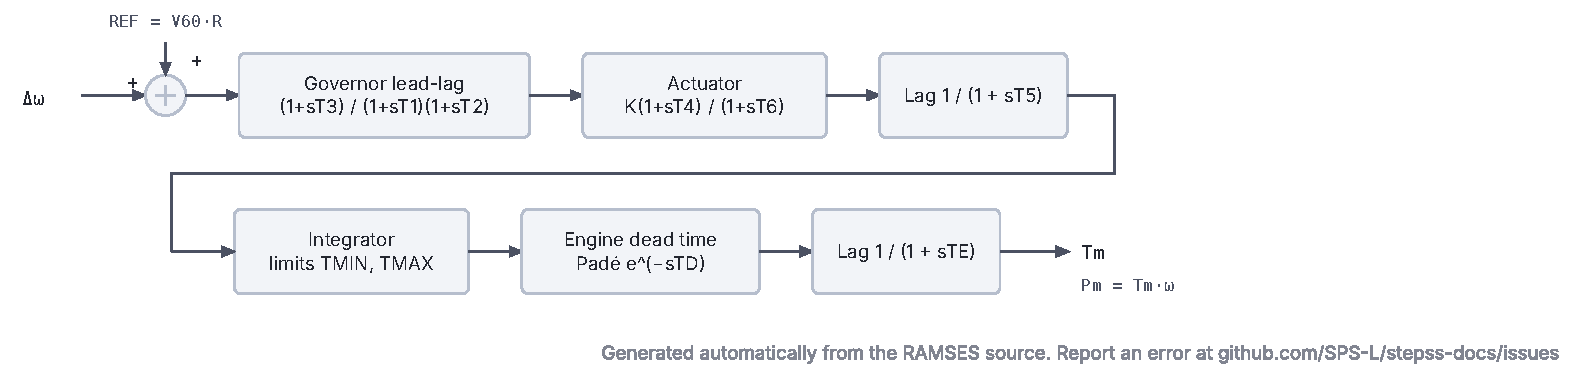
\includegraphics[width=0.98\linewidth]{figures/tor-degov1-light}
\caption{DEGOV1 block diagram.}
\end{figure}

\subsection{Parameters}\label{model-tor-ieee:parameters}

\begin{small}\begin{longtable}[]{@{}
  >{\raggedright\arraybackslash}p{(\linewidth - 4\tabcolsep) * \real{0.2266}}
  >{\raggedright\arraybackslash}p{(\linewidth - 4\tabcolsep) * \real{0.7734}}
@{}}
\toprule\noalign{}
\begin{minipage}[b]{\linewidth}\raggedright
Parameter
\end{minipage} & \begin{minipage}[b]{\linewidth}\raggedright
Description
\end{minipage} \\
\midrule\noalign{}
\endhead
\bottomrule\noalign{}
\endlastfoot
\texttt{SWM} & Input switch: 0 = mechanical torque (\(T_m\)), 1 = electrical power (\(P\)) \\
\texttt{T1} & Governor time constant, lead numerator (s) \\
\texttt{T2} & Governor time constant, lag denominator (s) \\
\texttt{T3} & Governor time constant, second-order denominator (s) \\
\texttt{K} & Actuator gain \\
\texttt{T4} & Actuator lead time constant (s) \\
\texttt{T5} & First-order actuator lag (s) \\
\texttt{T6} & Actuator lag time constant (s) \\
\texttt{TMIN} & Minimum fuel/torque limit (pu) \\
\texttt{TMAX} & Maximum fuel/torque limit (pu) \\
\texttt{TD} & Engine dead time (s) \\
\texttt{R} & Speed droop (pu/pu) \\
\texttt{TE} & Engine time constant (s) \\
\end{longtable}\end{small}

\textbf{Internal parameters:} \texttt{V60} (selected reference input, mechanical torque or electrical power according to \texttt{SWM}) and \texttt{REF} (\texttt{V60\ \ensuremath{\cdot}\ R}), both set at initialisation

\subsection{Usage Example}\label{model-tor-ieee:usage-example}

\textbf{RAMSES Data File}

\begin{Verbatim}
SYNC_MACH g1  g1  1. 1.  0.  0.   600. 570. 6. 0. 2.05
                    XT   0.15  2.2  0.3   0.2   2.   0.4  0.2  0.1  6.0257  0.  7.00  0.05  1.5  0.05
              EXC GENERIC1   3.0618 -0.1  1.  0.  100. -1. -20.0  10.  120. 5.  12.5 0.1  0.  5.
                                1     75.   15.    0.22    0.012     0.22    0.012    -0.1    0.1
              TOR DEGOV1  0      ! SWM: 0 = torque input, 1 = power input
                          0.02   ! T1: governor lead time constant (s)
                          0.02   ! T2: governor lag time constant (s)
                          0.20   ! T3: governor second-order denominator (s)
                          1.0    ! K: actuator gain
                          0.25   ! T4: actuator lead time constant (s)
                          0.009  ! T5: first-order actuator lag (s)
                          0.038  ! T6: actuator lag time constant (s)
                          0.0    ! TMIN: minimum fuel/torque limit (pu)
                          1.05   ! TMAX: maximum fuel/torque limit (pu)
                          0.01   ! TD: engine dead time (s)
                          0.05   ! R: speed droop (pu/pu)
                          0.05 ; ! TE: engine time constant (s)
\end{Verbatim}

\textbf{Notes}

\begin{itemize}
\tightlist
\item
  Set \texttt{SWM\ =\ 0} to use mechanical torque as the reference input, \texttt{SWM\ =\ 1} for electrical power.
\item
  \texttt{TMIN} and \texttt{TMAX} are per-unit limits on the integrator output (fuel demand / valve position).
\item
  \texttt{R} is the permanent droop; typical values are 0.04--0.05 pu/pu.
\item
  The Pad\'e approximation of the dead time \(T_D\) is a second-order filter.
\item
  Parameters are listed in order: \texttt{SWM\ T1\ T2\ T3\ K\ T4\ T5\ T6\ TMIN\ TMAX\ TD\ R\ TE}.
\end{itemize}

\begin{center}\rule{0.5\linewidth}{0.5pt}\end{center}

\section{\texorpdfstring{ENTSOE\_simp (\texttt{tor\_ENTSOE\_simp})}{ENTSOE\_simp (tor\_ENTSOE\_simp)}}\label{model-tor-ieee:entsoe_simp-tor_entsoe_simp}

\subsection{Scientific Description}\label{model-tor-ieee:scientific-description-1}

The \texttt{ENTSOE\_simp} model is a simplified \textbf{ENTSO-E speed governor} suitable for primary frequency response studies. It is derived from the ENTSO-E recommendations for equivalent turbine-governor representation.

The governor equation forms a speed error with permanent droop \(R\):

\[
R \cdot \dot{p}_1 - C + (\omega - 1) = 0, \quad C = T_m \cdot R
\]

This error drives a first-order lag (representing the valve or steam chest) with limits \([V_{MIN},\, V_{MAX}]\):

\[
\frac{d p_2}{dt} = \frac{1}{T_1}(p_1 - p_2), \quad p_2 \in [V_{MIN},\, V_{MAX}]
\]

The turbine mechanical power is modelled by a lead--lag transfer function with time constants \(T_2\) (zero) and \(T_3\) (pole):

\[
P_m(s) = \frac{1 + s T_2}{1 + s T_3} \cdot p_2(s)
\]

The final mechanical torque output accounting for shaft speed is:

\[
T_m \cdot \omega = P_m
\]

\begin{figure}[htbp]
\centering
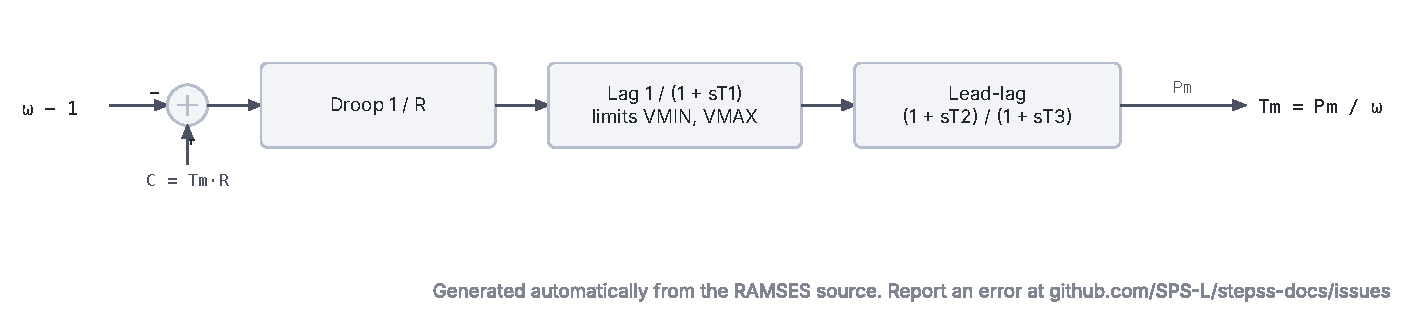
\includegraphics[width=0.98\linewidth]{figures/tor-entsoe-simp-light}
\caption{ENTSOE\_simp block diagram.}
\end{figure}

\subsection{Parameters}\label{model-tor-ieee:parameters-1}

\begin{small}\begin{longtable}[]{@{}ll@{}}
\toprule\noalign{}
Parameter & Description \\
\midrule\noalign{}
\endhead
\bottomrule\noalign{}
\endlastfoot
\texttt{R} & Permanent speed droop (pu/pu) \\
\texttt{T1} & Governor/valve time constant (s) \\
\texttt{VMIN} & Minimum valve position / lower output limit (pu) \\
\texttt{VMAX} & Maximum valve position / upper output limit (pu) \\
\texttt{T2} & Turbine lead time constant, zero (s) \\
\texttt{T3} & Turbine lag time constant, pole (s) \\
\end{longtable}\end{small}

\textbf{Internal parameter:} \texttt{C\ =\ Tm\ \ensuremath{\cdot}\ R} (initialised from the load-flow mechanical torque)

\subsection{Usage Example}\label{model-tor-ieee:usage-example-1}

\textbf{RAMSES Data File}

\begin{Verbatim}
SYNC_MACH g1  g1  1. 1.  0.  0.   400. 360. 6. 0. 2.05
                    XT   0.15  2.2  0.3   0.2   2.   0.4  0.2  0.1  6.0257  0.  7.00  0.05  1.5  0.05
              EXC GENERIC1   3.0618 -0.1  1.  0.  100. -1. -20.0  10.  120. 5.  12.5 0.1  0.  5.
                                1     75.   15.    0.22    0.012     0.22    0.012    -0.1    0.1
              TOR ENTSOE_simp  0.05   ! R: permanent droop (pu/pu)
                               0.50   ! T1: governor/valve time constant (s)
                               0.0    ! VMIN: minimum valve position (pu)
                               1.1    ! VMAX: maximum valve position (pu)
                               0.0    ! T2: turbine lead time constant (s)
                               10.0 ; ! T3: turbine lag time constant (s)
\end{Verbatim}

\textbf{Notes}

\begin{itemize}
\tightlist
\item
  Typical primary-frequency response studies use \(R = 0.04\)--\(0.05\).
\item
  Setting \(T_2 = 0\) simplifies the turbine to a pure first-order lag \(1/(1+sT_3)\).
\item
  This model is commonly used as a simplified equivalent for aggregated generation.
\item
  Parameters are listed in order: \texttt{R\ T1\ VMIN\ VMAX\ T2\ T3}.
\end{itemize}

\begin{center}\rule{0.5\linewidth}{0.5pt}\end{center}

\section{\texorpdfstring{GAST (\texttt{tor\_GAST})}{GAST (tor\_GAST)}}\label{model-tor-ieee:gast-tor_gast}

\subsection{Scientific Description}\label{model-tor-ieee:scientific-description-2}

The \texttt{GAST} model represents a \textbf{gas turbine} unit, following the IEEE Committee Report (1973) and the convention common to industry tools. It captures the speed governor, compressor discharge lag, and fuel/combustion dynamics.

\textbf{Speed governor with droop and load reference:}

\[
\text{error} = R \cdot (V_{act} - LR) + (\omega - 1) = 0
\]

where \(LR = T_m\) (load reference, initialised from mechanical torque) and \(R\) is the droop.

The speed error drives a value position through a limiter \([V_{MIN},\, V_{MAX}]\) and a first-order lag \(T_1\):

\[
\frac{d p_2}{dt} = \frac{1}{T_1}(p_1 - p_2)
\]

The compressor discharge is modelled by lag \(T_2\):

\[
\frac{d p_3}{dt} = \frac{1}{T_2}(p_2 - p_3)
\]

The mechanical power (including speed-dependent damping \(D_{TURB}\)) is:

\[
P_m = p_3 + D_{TURB} \cdot (\omega - 1)
\]

The exhaust temperature is tracked by a lag \(T_3\):

\[
\frac{d p_4}{dt} = \frac{1}{T_3}(p_3 - p_4)
\]

A temperature limit is applied via:

\[
p_5 = A_T + K_T \cdot (A_T - p_4)
\]

A minimum gate blocks the valve position: \(p_1 = \min(p_{gov},\, p_5)\).

The torque-power conversion:

\[
T_m \cdot \omega = P_m
\]

\begin{figure}[htbp]
\centering
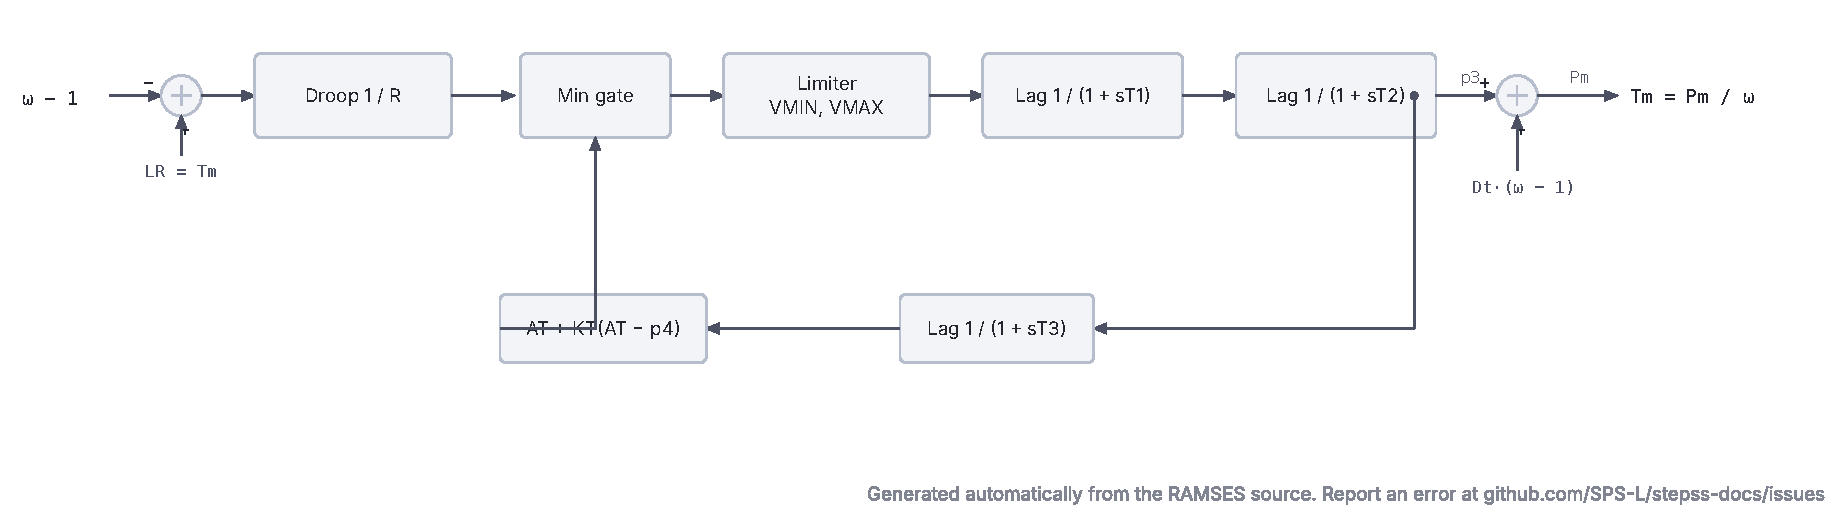
\includegraphics[width=0.98\linewidth]{figures/tor-gast-light}
\caption{GAST block diagram.}
\end{figure}

\subsection{Parameters}\label{model-tor-ieee:parameters-2}

\begin{small}\begin{longtable}[]{@{}ll@{}}
\toprule\noalign{}
Parameter & Description \\
\midrule\noalign{}
\endhead
\bottomrule\noalign{}
\endlastfoot
\texttt{R} & Permanent speed droop (pu/pu) \\
\texttt{T1} & Governor/valve time constant (s) \\
\texttt{T2} & Compressor discharge time constant (s) \\
\texttt{T3} & Radiation shield / exhaust temperature lag (s) \\
\texttt{AT} & Ambient temperature load limit (pu) \\
\texttt{KT} & Temperature control loop gain \\
\texttt{VMAX} & Maximum valve position (pu) \\
\texttt{VMIN} & Minimum valve position (pu) \\
\texttt{DTURB} & Turbine damping factor (pu torque / pu speed) \\
\end{longtable}\end{small}

\textbf{Internal parameter:} \texttt{LR\ =\ Tm} (load reference, set at initialisation)

\subsection{Usage Example}\label{model-tor-ieee:usage-example-2}

\textbf{RAMSES Data File}

\begin{Verbatim}
SYNC_MACH g1  g1  1. 1.  0.  0.   400. 360. 6. 0. 2.05
                    XT   0.15  2.2  0.3   0.2   2.   0.4  0.2  0.1  6.0257  0.  7.00  0.05  1.5  0.05
              EXC GENERIC1   3.0618 -0.1  1.  0.  100. -1. -20.0  10.  120. 5.  12.5 0.1  0.  5.
                                1     75.   15.    0.22    0.012     0.22    0.012    -0.1    0.1
              TOR GAST  0.05   ! R: permanent droop (pu/pu)
                        0.40   ! T1: governor/valve time constant (s)
                        0.10   ! T2: compressor discharge time constant (s)
                        3.00   ! T3: exhaust temperature lag (s)
                        1.00   ! AT: ambient temperature load limit (pu)
                        2.50   ! KT: temperature control loop gain
                        1.05   ! VMAX: maximum valve position (pu)
                        0.0    ! VMIN: minimum valve position (pu)
                        0.0  ; ! DTURB: turbine damping factor
\end{Verbatim}

\textbf{Notes}

\begin{itemize}
\tightlist
\item
  Based on the IEEE Committee Report on ``Dynamic Models for Steam and Hydro Turbines in Power System Studies'' (1973), later adapted for gas turbines.
\item
  \texttt{AT} and \texttt{KT} define the exhaust-temperature protection characteristic.
\item
  \texttt{DTURB\ =\ 0} disables speed-dependent damping.
\item
  Parameters are listed in order: \texttt{R\ T1\ T2\ T3\ AT\ KT\ VMAX\ VMIN\ DTURB}.
\end{itemize}

\begin{center}\rule{0.5\linewidth}{0.5pt}\end{center}

\section{\texorpdfstring{TGOV1 (\texttt{tor\_TGOV1D})}{TGOV1 (tor\_TGOV1D)}}\label{model-tor-ieee:tgov1-tor_tgov1d}

\subsection{Scientific Description}\label{model-tor-ieee:scientific-description-3}

The \texttt{TGOV1} model represents a \textbf{simple steam turbine governor}, based on the IEEE TGOV1 structure with an added damping term. It is one of the most widely used simple governor models in power-system stability studies.

\textbf{Speed governor with permanent droop:}

The speed error (with droop \(R\)) drives a first-order lag \(T_1\) with output limits \([V_{MIN},\, V_{MAX}]\):

\[
R \cdot p_1 - C + (\omega - 1) = 0, \quad C = T_m \cdot R
\]

\[
\frac{d p_2}{dt} = \frac{1}{T_1}(p_1 - p_2), \quad p_2 \in [V_{MIN},\, V_{MAX}]
\]

\textbf{Turbine with reheater and damping:}

The valve position passes through a lead--lag block representing the steam chest and reheater:

\[
P_m(s) = \frac{1 + s T_2}{1 + s T_3} \cdot p_2(s)
\]

The total mechanical power includes a speed-dependent damping term \(D_t\):

\[
P_m = p_{turbine} + D_t \cdot (\omega - 1)
\]

Hence the mechanical torque:

\[
T_m = \frac{P_m}{\omega}
\]

\begin{figure}[htbp]
\centering
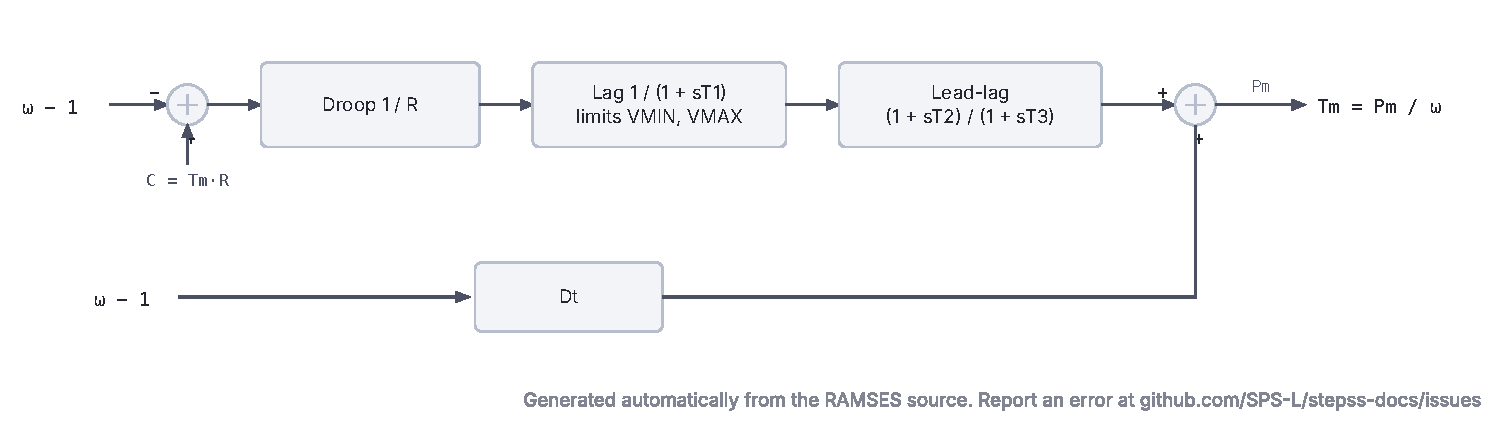
\includegraphics[width=0.98\linewidth]{figures/tor-tgov1-light}
\caption{TGOV1 block diagram.}
\end{figure}

\subsection{Parameters}\label{model-tor-ieee:parameters-3}

\begin{small}\begin{longtable}[]{@{}ll@{}}
\toprule\noalign{}
Parameter & Description \\
\midrule\noalign{}
\endhead
\bottomrule\noalign{}
\endlastfoot
\texttt{R} & Permanent speed droop (pu/pu) \\
\texttt{T1} & Steam chest / valve actuator time constant (s) \\
\texttt{VMAX} & Maximum valve position (pu) \\
\texttt{VMIN} & Minimum valve position (pu) \\
\texttt{T2} & Lead time constant, reheater zero (s) \\
\texttt{T3} & Lag time constant, reheater pole (s) \\
\texttt{Dt} & Turbine damping coefficient (pu torque / pu speed deviation) \\
\end{longtable}\end{small}

\textbf{Internal parameter:} \texttt{C\ =\ Tm\ \ensuremath{\cdot}\ R} (initialised from load-flow mechanical torque)

\subsection{Usage Example}\label{model-tor-ieee:usage-example-3}

\textbf{RAMSES Data File}

\begin{Verbatim}
SYNC_MACH g1  g1  1. 1.  0.  0.   400. 360. 6. 0. 2.05
                    XT   0.15  2.2  0.3   0.2   2.   0.4  0.2  0.1  6.0257  0.  7.00  0.05  1.5  0.05
              EXC GENERIC1   3.0618 -0.1  1.  0.  100. -1. -20.0  10.  120. 5.  12.5 0.1  0.  5.
                                1     75.   15.    0.22    0.012     0.22    0.012    -0.1    0.1
              TOR TGOV1  0.05   ! R: permanent droop (pu/pu)
                          0.50   ! T1: steam chest/valve actuator time constant (s)
                          1.05   ! VMAX: maximum valve position (pu)
                          0.0    ! VMIN: minimum valve position (pu)
                          2.10   ! T2: lead time constant, reheater zero (s)
                          7.00   ! T3: lag time constant, reheater pole (s)
                          0.0  ; ! Dt: turbine damping coefficient
\end{Verbatim}

\textbf{Notes}

\begin{itemize}
\tightlist
\item
  This is essentially the IEEE TGOV1 model with an additional damping term \(D_t\).
\item
  Setting \(T_2 = 0\) gives a pure first-order turbine \(1/(1+sT_3)\).
\item
  \(D_t > 0\) adds a stabilising speed-dependent power correction (useful for islanded operation).
\item
  Parameters are listed in order: \texttt{R\ T1\ VMAX\ VMIN\ T2\ T3\ Dt}.
\end{itemize}

\begin{center}\rule{0.5\linewidth}{0.5pt}\end{center}

\section{\texorpdfstring{HYGOV (\texttt{tor\_hygov})}{HYGOV (tor\_hygov)}}\label{model-tor-ieee:hygov-tor_hygov}

\subsection{Scientific Description}\label{model-tor-ieee:scientific-description-4}

The \texttt{HYGOV} model represents a \textbf{hydraulic turbine and governor} following a simplified penstock/water-column formulation, consistent with the IEEE representation for hydro governors (IEEE Std 1110).

\textbf{Governor with droop and PI controller:}

The speed error (with permanent droop \(R\) and transient droop \(r\)) enters a lag \(T_f\) to produce the error signal \(e\):

\[
\text{input} = 1 - \omega - R \cdot (c - P_0)
\]

\[
\frac{d e}{dt} = \frac{1}{T_f}\left(\text{input} - e\right)
\]

The rate of change of gate demand is computed via the transient droop:

\[
\dot{x}_2 = \frac{e}{r \cdot T_r}
\]

This is rate-limited to \([-V_{ELM},\, +V_{ELM}]\), then integrated with gate limits \([G_{min},\, G_{max}]\):

\[
\frac{d x_4}{dt} = x_3, \quad x_4 \in [G_{min},\, G_{max}]
\]

The PI controller output (desired gate) is:

\[
x_5 = x_4 + \frac{e}{r}, \quad c = \text{clip}(x_5,\, G_{min},\, G_{max})
\]

The actual gate position follows through the servo:

\[
\frac{d g}{dt} = \frac{1}{T_g}(c - g)
\]

\textbf{Penstock / water column:}

The head deviation \(dH\) is determined by the non-linear water flow equation and water-starting time \(T_W\):

\[
1 - \left(\frac{Q}{g}\right)^2 = dH
\]

\[
T_W \cdot \frac{dQ}{dt} = dH
\]

\textbf{Turbine mechanical torque:}

\[
T_m \cdot \omega = A_t \cdot (1 - dH)(Q - Q_{nl}) - D_{turb} \cdot (1 - \omega) \cdot g
\]

\[
P_m = T_m \cdot \omega
\]

\begin{figure}[htbp]
\centering
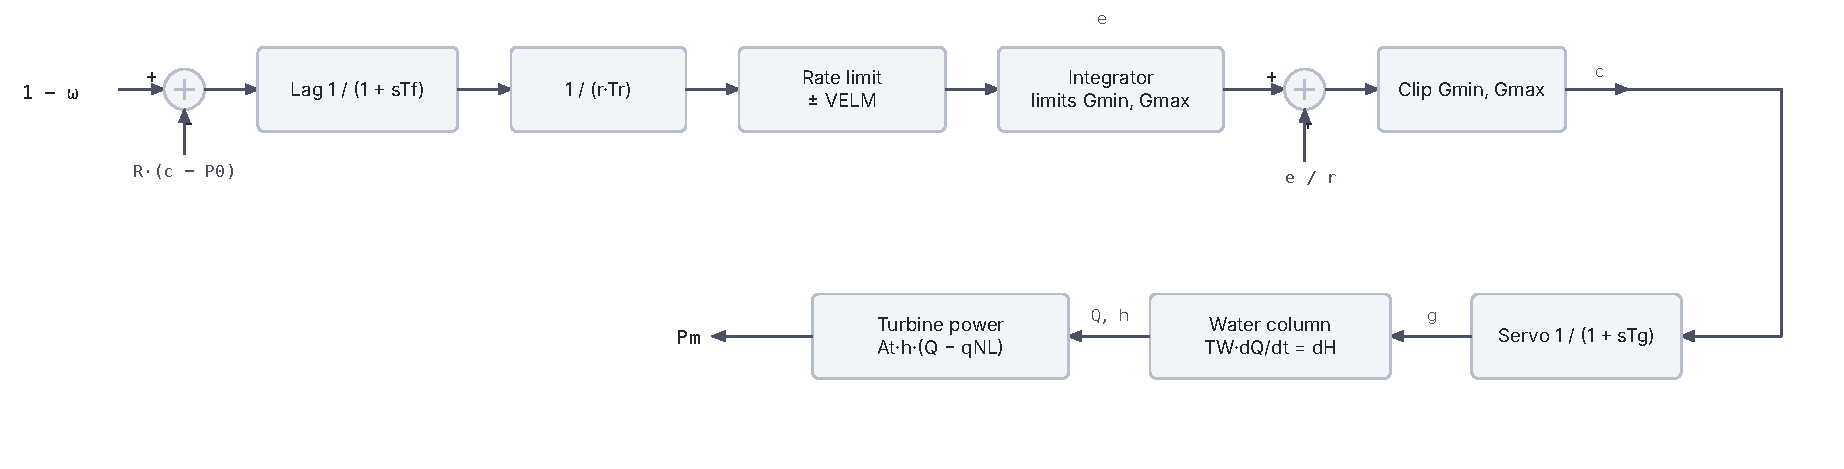
\includegraphics[width=0.98\linewidth]{figures/tor-hygov-light}
\caption{HYGOV block diagram.}
\end{figure}

\subsection{Parameters}\label{model-tor-ieee:parameters-4}

\begin{small}\begin{longtable}[]{@{}ll@{}}
\toprule\noalign{}
Parameter & Description \\
\midrule\noalign{}
\endhead
\bottomrule\noalign{}
\endlastfoot
\texttt{R} & Permanent droop (pu/pu) \\
\texttt{r} & Transient droop (pu/pu) \\
\texttt{Tr} & Transient droop reset time (s) \\
\texttt{Tf} & Filter time constant for speed error (s) \\
\texttt{Tg} & Gate servo time constant (s) \\
\texttt{VELM} & Gate velocity limit (pu/s) \\
\texttt{Gmax} & Maximum gate opening (pu) \\
\texttt{Gmin} & Minimum gate opening (pu) \\
\texttt{Tw} & Water starting time (s) \\
\texttt{At} & Turbine gain (pu power / pu flow) \\
\texttt{Dturb} & Turbine damping factor \\
\texttt{Qnl} & No-load water flow (pu) \\
\end{longtable}\end{small}

\textbf{Internal parameter:} \texttt{Po\ =\ (P\ /\ At)\ +\ Qnl} (initial gate setpoint from load-flow)

\subsection{Usage Example}\label{model-tor-ieee:usage-example-4}

\textbf{RAMSES Data File}

\begin{Verbatim}
SYNC_MACH g1  g1  1. 1.  0.  0.   800. 760. 3. 0. 0.95
                    XT   0.15  1.1  0.25  0.2  0.7  *  0.2  0.1  6.0257  0.  5.00  0.05  *  0.1
              EXC GENERIC1   1.8991 -0.1  0.  1.  100. -1. -11  10.  70.  10.  20. 0.1  0.  4.
                                1     75.   15.    0.2    0.01     0.2    0.01    -0.1    0.1
              TOR HYGOV  0.05   ! R: permanent droop (pu/pu)
                         0.30   ! r: transient droop (pu/pu)
                         5.00   ! Tr: transient droop reset time (s)
                         0.05   ! Tf: filter time constant for speed error (s)
                         0.20   ! Tg: gate servo time constant (s)
                         0.20   ! VELM: gate velocity limit (pu/s)
                         1.00   ! Gmax: maximum gate opening (pu)
                         0.0    ! Gmin: minimum gate opening (pu)
                         1.50   ! Tw: water starting time (s)
                         1.10   ! At: turbine gain (pu power / pu flow)
                         0.50   ! Dturb: turbine damping factor
                         0.05 ; ! Qnl: no-load water flow (pu)
\end{Verbatim}

\textbf{Notes}

\begin{itemize}
\tightlist
\item
  \texttt{Tw} (water starting time) is the dominant parameter controlling frequency response; typical values are 0.5--2 s.
\item
  \texttt{r\ \textgreater{}\ R} is required for stable regulation; set \(r \approx 2\)--5 \(\times R\).
\item
  \texttt{Tr} is the reset time for transient droop; values of 5--30 s are typical.
\item
  Non-linear head-flow equation makes this model suitable for large transients.
\item
  Parameters are listed in order: \texttt{R\ r\ Tr\ Tf\ Tg\ VELM\ Gmax\ Gmin\ Tw\ At\ Dturb\ Qnl}.
\end{itemize}
